%!TEX program = lualatex

% https://github.com/tudace/tuda_latex_templates/issues/472#issuecomment-2203339479
\DocumentMetadata{
	pdfstandard=a-2b,
	% TODO: Change to "en" if you write in English
	lang=de,
	pdfversion=1.7,
}

\documentclass[
	ngerman,
	ruledheaders=section,%Ebene bis zu der die Überschriften mit Linien abgetrennt werden, vgl. DEMO-TUDaPub
	class=report,%Basisdokumentenklasse. Wählt die Korrespondierende KOMA-Script Klasse
	thesis={type=master},%Dokumententyp Thesis, für Dissertationen siehe die Demo-Datei DEMO-TUDaPhd
	accentcolor=1b,%Auswahl der Akzentfarbe
	custommargins=false,% Ränder werden mithilfe von typearea automatisch berechnet
	marginpar=false,% Kopfzeile und Fußzeile erstrecken sich nicht über die Randnotizspalte
	BCOR=12mm,%Bindekorrektur, falls notwendig
	parskip=half-,%Absatzkennzeichnung durch Abstand vgl. KOMA-Sript
	fontsize=11pt,%Basisschriftgröße laut Corporate Design ist mit 9pt häufig zu klein
	IMRAD=false,%Abschalten von IMRAD-Warnings wegen fehlender Labels
]{tudapub}

% Der folgende Block ist nur bei pdfTeX auf Versionen vor April 2018 notwendig
\usepackage{iftex}
\ifPDFTeX
\usepackage[utf8]{inputenc}%kompatibilität mit TeX Versionen vor April 2018
\fi

%%%%%%%%%%%%%%%%%%%
%Sprachanpassung und Verbesserte Trennregeln
%%%%%%%%%%%%%%%%%%%
\usepackage[english, main=ngerman]{babel}
\usepackage{microtype}

%%%%%%%%%%%%%%%%%%%
%Tabellen
%%%%%%%%%%%%%%%%%%%
%\usepackage{array}     % Basispaket für Tabellenkonfiguration, wird von den folgenden automatisch geladen
%\usepackage{tabularx}  % Tabellen, die sich automatisch der Breite anpassen
%\usepackage{longtable} % Mehrseitige Tabellen
%\usepackage{xltabular} % Mehrseitige Tabellen mit anpassarer Breite
\usepackage{booktabs}   % Verbesserte Möglichkeiten für Tabellenlayout über horizontale Linien

%%%%%%%%%%%%%%%%%%%
%Paketvorschläge Mathematik
%%%%%%%%%%%%%%%%%%%
\usepackage{mathtools}  % erweiterte Fassung von amsmath
\usepackage{amssymb}    % erweiterter Zeichensatz
%\usepackage{siunitx}   % Einheiten

\renewcommand{\thefigure}{\arabic{figure}} % fortlaufende Nummerierung von Abbildungen (nur für die Aufgabenstellung nutzen!)

\usepackage{lipsum} % Blindext im Beispiel erzeugen (kann entfernt werden)

%%%%%%%%%%%%%%%%%%%
%Beschriftung von Tabellen, Skizzen, Listings etc.
%%%%%%%%%%%%%%%%%%%
\usepackage{caption}
\captionsetup{justification=centering}



\begin{document}

\frontmatter

\Metadata{
	title=Hier steht der mehrzeilige Titel der Thesis,
	author=Jane Doe
}

\title{Hier steht der mehrzeilige Titel der Thesis}
\subtitle{This is the English Title of the Thesis} %oder der deutsche Titel, falls Thesis in englisch geschrieben wird
\author[J. Doe]{Jane Doe}
\reviewer{Prof.~Dr.~rer.~nat.~Andy Schürr \and Erika Mustermann,~M.\,Sc.}%Gutachter

\department{etit}
\group{Fachgebiet Echtzeitsysteme}

\submissiondate{\today}
\examdate{\today}

\maketitle

\mainmatter

\chapter*{Aufgabenstellung}

\section*{Motivation}

Hier steht die Motivation und der State of the Art.
Diese Gliederung der Aufgabenstellung ist nur ein Vorschlag.
Dieser Satz ist ein Beispiel für das Zitieren von mehreren Quellen~\cite{Luthmann2017,Luthmann2019,Ruland2018}.
Der folgende Text ist Blindtext des Pakets \texttt{lipsum}.
\lipsum[1]

Ein Absatz wird durch eine Leerzeile erzeugt.
\lipsum[2]



\section*{Konzept}

Hier wird die angedachte Lösung für das motivierte Problem erläutert.
Dies ist ein Verweis auf Abbildung~\ref{fig:some-figure}.
\lipsum[3]

\begin{figure}[tp]
    \centering
    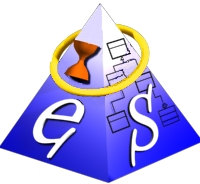
\includegraphics[width=.3\linewidth]{figures/es_logo_gross.jpg}
    \caption{Dies ist eine Beispiel-Abbildung, die das Logo der TU Darmstadt zeigt.}\label{fig:some-figure}
\end{figure}



\section*{Zielsetzungen}

Hier wird ein knapper, konkreter Überblick über die Zielsetzungen der Thesis vorgestellt.
Dabei kann es helfen, eine Übersichtsgrafik zu verwenden und Forschungsfragen zu formulieren.
\lipsum[4]



\bibliographystyle{plain}
\bibliography{chapters/references}
	
\end{document}